%%%%%%%%%%%%%%%%%%%%%%%%%%%%%%%%%%%%%%%%%%%%%%%%%%%%%%%%%%%%%%%%%%%%%%%%%%%%%%%%%%%%%%%%%%%%%%%%%%%%
%
% NOTE TO AIP TYPSETERS: TO CONVERT FROM TWO-COL TO PREPRINT, SWITCH
% COMMENTOUT COMMAND FROM A TO B IE. use
% \newcommand{\commentoutA}[1]{}
% \newcommand{\commentoutB}[1]{#1}
% instead of the following
\newcommand{\commentoutA}[1]{#1}
\newcommand{\commentoutB}[1]{}
\renewcommand{\thefootnote}{\fnsymbol{footnote}}

\commentoutA{\documentclass[prl,aps,twocolumn,showpacs,twocolumngrid,superbib]{revtex4}}
\commentoutB{\documentclass[prb,aps,nobibnotes,showpacs,superbib,preprint]{revtex4}}

\usepackage{graphicx}
\usepackage{amsfonts}
\usepackage{amsmath}
\usepackage{bm}
\usepackage{alltt}
%\usepackage{epsfig}
%%
%%

\begin{document}

\date{\today}

\title{Trace Re-Setting Density Matrix Purification in ${\cal O}(N)$ Self-Consistent-Field Theory\footnotemark[4] }

\author{Anders~M.~N.~Niklasson\footnotemark[2]}
\author{C.~J.~Tymczak\footnotemark[3]}
\author{Matt Challacombe\footnotemark[6]}
\affiliation{
Theoretical Division, Los Alamos National Laboratory,
Los Alamos, NM 87545, USA}

\begin{abstract}
A new approach to linear scaling construction of the density matrix is proposed,
based on Trace Re-Setting purification of an effective Hamiltonian.  Trace Re-Setting 
is related to the trace preserving canonical purification scheme of Palser and Manolopoulos 
[Phys.~Rev.~B, {\bf 58} 12704 (1999)] in that they both work with a predefined 
occupation number and do not require adjustment or prior knowledge of the chemical 
potential.  In the Trace Re-Setting approach, trace conservation is not strictly enforced, allowing 
greater flexibility in the choice of purification polynomial.  However, optimal polynomials 
may in some cases admit unstable solutions, requiring ``Trace Re-Setting'' mechanisms 
to bring the solution back into the domain of convergent purification.  
In the Trace Re-Setting method, use of an optimal polynomial allows greatly 
improved performance for Hamiltonian systems with high or low filling 
$f_{\rm occ}$.  A quartic Trace Re-Setting method is developed, along with analysis of 
stability and error accumulation due to incomplete sparse-matrix methods that employ a threshold $\tau$ 
to achieve sparsity.  It is argued that threshold induced purification errors in the 
density matrix scale ${\cal O}(\tau \Delta g^{-1})$ at worst, where $\Delta g$ is the gap at 
the chemical potential.  In the low filling regime,  purification derived total energies 
are shown to converge smoothly with $\tau^2$ for RPBE/STO-6G C60 and a RPBE0/STO-3G Ti 
substituted zeolite.  For the zeolite, the quartic Trace Re-Setting method is found to be 
both faster and over an order of magnitude more accurate than the Palser-Manolopoulos method.  In the low 
filling limit, true linear scaling is demonstrated for RHF/6-31G**  water clusters, and the 
Trace-Re-Setting method is found to be both faster and an order of magnitude more accurate 
than the Palser-Manolopoulos scheme.  Basis set progression of RPBE chlorophyll reveals the quartic 
Trace Re-Setting to be up to four orders of magnitude more accurate than the Palser-Manolopoulos algorithm
in the limit of low filling.

\smallskip
\noindent{\bf Keywords}: Self-Consistent-Field, Density Functional Theory, Hartree-Fock, Gaussian-Orbital, 
                         Linear-Scaling, Density Matrix, Spectral Projection, Purification, Sparse Matrix
\end{abstract}

\pacs{02.60.Dc,31.15.Ne,71.15Dx,71.15Nc}

%\keywords{Self-Consistent-Field,linear-scaling,density matrix,spectral projection,purification,sparse matrix,AINV,Gaussian-Orbital}

\maketitle

\footnotetext[2]{\tt amn@LANL.Gov}
\footnotetext[3]{\tt Tymczak@LANL.Gov}
\footnotetext[6]{\tt MChalla@LANL.Gov}
\footnotetext[4]{Preprint LA-UR-02-6997.}

\section{Introduction}

For non-metallic systems it is now possible to solve the Self-Consistent-Field (SCF)
equations for systems with thousands of atoms using linear scaling methods. These methods 
achieve a reduced ${\cal O}(N)$ computational complexity, where $N$ is the number of basis 
functions assumed proportional to system size. In contrast, conventional formulations of 
Self-Consistent-Field theory, such as the Roothaan-Hall \cite{CRoothaan51,GHall51} and Kohn-Sham \cite{WKohn65} 
method, involve ${\cal O}(N^3)$ eigensolution of the effective single-particle Hamiltonian or Fockian 
$\bf F$ in an orthogonal representation;
\begin{equation}\label{EigenvalueProblem}
\bf F C = \bf e \bf C.
\end{equation}
The matrix of eigenvectors $\bf C$ is spanned by the molecular orbitals ${\bf c}_k$ (the eigenvectors), from which
the first order reduced density matrix is constructed via the outer product
\begin{equation}\label{DensityFromMOs}
{\bf P} = \sum_{k=1}^{N_{\rm el}} {\bf c}^{\rm T}_{k} {\bf c}_{k}.
\end{equation}
The eigenvalues $e_i$ determine the electronic single-particle energy
\begin{subequations}
\begin{eqnarray} 
E_{\rm el} &=& \sum_{i=1}^{N_{\rm el}} e_i \label{EigenEnergy}  \\
&=&{\rm Tr}[ \bf P F ], \label{TraceEnergy} 
\end{eqnarray}
\end{subequations}
with $N_{\rm el}$ the number of occupied electronic states.
This approach to solving the SCF equations using hybrid Hartree-Fock/Density Functional Theory,
Hartree-Fock (Roothaan-Hall) or  pure Density Functional Theory (Kohn-Sham) will, in the following, 
be referred to interchangeably as eigensolution (ES).

Many of the linear scaling methods involve iterative construction of the density matrix 
in a local, non-orthogonal basis, exploiting the approximately exponential decay 
\cite{WKohn59,JCloizeaux64,PMaslen98,SIsmail99,XZhang01,STaraskin99}
of matrix elements with basis function separation through the use of sparse matrix technologies.  
These technologies include linear algebra kernels such as sparse matrix-matrix multiplication
and incomplete methods for computing congruence transformations between orthogonal and 
non-orthogonal representations.

One approach to constructing the density matrix is via functional minimization of an
energy like expression related to Eq.(\ref{TraceEnergy})
% Is this really a minimization method? ASameh82: 
\cite{ASameh82,XLi93,ACarlsson95,EHernandez96,WKohn96,ADaniels97,UStephan98,MChallacombe99,PHaynes99,DBowler99,ADaniels99}.
This is the density matrix minimization (DMM) approach. 
A second approach is via polynomial approximation of
\begin{equation}
\label{Heavyside}
\bf P = \theta ( \mu \bf I - \bf F ),
\end{equation}
where $\theta$ is the Heavyside step function (or the Fermi-Dirac distribution) setting all eigenvalues
above the chemical potential $\mu$ to $0$ and all the occupied eigenvalues below $\mu$ to $1$,
forming an idempotent density matrix 
\cite{RMcWeeny60,APalser99,MChallacombe99,DBowler99,ADaniels99,Goedecker94,CKenney95,GBeylkin99,AHolas01,ANiklasson02A,ANiklasson02B}.
This is the polynomial expansion (PE) or spectral projection approach.
Both the functional minimization and the spectral projection methods 
can be posed as a general expansion of the density matrix in terms of 
the Fockian, {\em i.e.} $\bf P = {\cal P}(F)$ for some polynomial ${\cal P}$.
In an iterative approach this expansion can be formulated as
\begin{subequations}
\begin{eqnarray}
&& {\bf X}_0 = {\cal P}_{0}(\bf F) \\
&& {\bf X}_{n+1} = {\cal P}_{n+1}({\bf F}, {\bf X}_n) ~~ {\rm (DMM)} \label{DMMPoly}\\
&& {\bf X}_{n+1} = {\cal P}_{n+1}({\bf X}_n)~~~~~~~~ {\rm  (PE)} \label{PEPoly}\\
&& {\bf P} = \lim_{n \rightarrow \infty} {\bf X}_n.
\end{eqnarray}
\end{subequations}

There is a subtle distinction between polynomial expansion (PE) and density 
matrix minimization (DMM) due to the use of approximate sparse matrix algebra, wherein
sparsity is enforced through a radial cutoff or numerical threshold  to 
achieve $N$-scaling of the sparse matrix-matrix multiply. In polynomial expansion schemes, 
such as density matrix purification, 
this approximate sparse-matrix algebra leads to an {\em accumulated error} in the density matrix 
that is separate from and additional to the {\em truncation error}.  We define truncation error as the 
error resulting simply from dropping elements of the exact density matrix.  Density matrix 
minimization methods such as the Li-Nunes-Vanderbilt \cite{XLi93,DBowler99} (LNV) approach are able to 
avoid accumulation errors through continued use of gradient expressions that contain the Fockian, 
as implied by Eq.~(\ref{DMMPoly}). On the other hand, polynomial expansion methods lose contact 
with the Fockian after the first iteration, allowing repeated iterations with 
approximate sparse matrix algebra to blur the eigenbasis.  However, density matrix purification 
methods tend to be more efficient than density matrix minimization methods, requiring fewer 
matrix-multiplies and converging quadratically as they reach idempotence.

There are a number density matrix purification schemes worth differentiating amongst: 
{\it 1)} {\it Grand Canonical} schemes, with a step function  expansion around a predefined 
         chemical potential \cite{RMcWeeny60,APalser99,AHolas01,ANiklasson02A,ANiklasson02B},
{\it 2)} {\it Canonical Trace Conserving} schemes, with a fixed trace
         in each iteration step \cite{APalser99}, 
{\it 3)} {\it Trace Correcting} methods, where the trace reaches the correct value only at 
         convergence \cite{ANiklasson02A}, and finally 
{\it 4)} {\it Trace Re-Setting} algorithms (this article), where trace is not rigorously conserved,
          requiring a resetting  mechanism if the domain of convergence is exceeded.
There are also various hybrid approaches that mix both density matrix minimization and 
purification together.  For example Challacombe \cite{MChallacombe99} used a commuting 
 minimization scheme to precondition a grand canonical purification scheme,
while Bowler \cite{DBowler99} suggests the use of the LNV density matrix minimization 
after purification to reduce accumulation errors.

Perhaps most closely related to the present work, a canonical trace 
conserving purification scheme was recently constructed by Palser and Manolopoulos 
(PM) in Ref.~\onlinecite{APalser99}. 
By using a starting guess ${\bf X}_0$ with the trace equal to 
the occupation number and thereafter performing trace-conserving
spectral projections, ${\bf X}_n$ converges to the correct density matrix without
prior knowledge of the chemical potential. 

The PM scheme has an excellent performance compared to other methods \cite{APalser99,ADaniels99,GBerghold02,YShao02}, and is also
able to deal with degenerate eigensystems and fractional occupancy.  However, application of PM has failed 
in the case of semi-empirical methods, most notably for C60, where convergence to excited states and 
other problems were encountered \cite{ADaniels99}.   Also, due to accumulation errors, PM is 
not variational when applied to non-self-consistent theories such as tight binding \cite{APalser99,DBowler99}.
Relevant to {\it ab initio} SCF methods, trace conservation leads to  inefficiencies at low 
and high filling, $f_{occ}=N_e/N$, due to the unfavorable behavior of ${\cal P}_{\rm PM}$ near 
its endpoints \cite{APalser99,ANiklasson02A}.  Low filling $f_{occ}\lesssim .2$  is encountered 
with a large basis set, while high filling $f_{occ} \gtrsim .8$ corresponds to a small basis set.

In this paper, we introduce a new Trace Re-Setting purification scheme (TRS) 
that is efficient for high and low fillings.  This new method is 
efficient because it employs a polynomial that is uniformly well behaved, but with the
potential for violating trace conservation in intermediate steps.  The method can deal with
degeneracy and converges more rapidly for both small and large basis sets, significantly reducing 
accumulation errors due to threshold induced blurring of the eigenbasis.

The outline of this paper follows:  In Section \ref{TSP}, we define Trace Re-Setting purification,
and present a fourth order algorithm.  Then, in Appendix \ref{Degen} we discuss the ability of
Trace Re-Setting methods to cope with degenerate eigensystems and fractional occupancy.  In Section 
\ref{Error}, we analyze the asymptotic behavior of the initial accumulated errors, and their stability 
at idempotence.  Finally, the new Trace Re-Setting algorithm is compared 
to the PM scheme and exact eigensolution on the basis of accuracy and time to convergence.

\section{Purification}\label{TSP}

The general idea behind purification for construction 
of the density matrix is based on an iterative expansion of the
Fockian in terms of a continuously increasing 
polynomial ${\cal P}(x)$, $x \in [0,1]$  with fixed end point extrema
%stationary fixed end points extremums WMC
at $0$ and $1$, i.e. ${\cal P}(0) = 0$, ${\cal P}(1) = 1$, and ${\cal P}'(0)={\cal P}'(1)=0$. 
It can be shown that a nested sequence of such polynomials 
converges to a step function with a step somewhere in $[0,1]$. 
First we discuss the grand canonical McWeeny method and the canonical
purification scheme before presenting the main ideas of Trace Re-Setting purification.

\subsection{McWeeny Purification}

The grand canonical McWeeny purification scheme \cite{RMcWeeny60,APalser99}
is a polynomial expansion based on the following iteration:
\begin{equation} \label{P3}
{\bf X}_{n+1} = {\cal P}_{\rm McW}({\bf X}_n) = 3 {\bf X}_n^2 - 2 {\bf X}_n^3, ~~~~~ n = 0,1,2, \ldots
\end{equation}
using the initial guess 
\begin{equation} \label{Pur2}
{\bf X}_0 = \alpha(\mu { \bf I} - {\bf F}) + \beta{ \bf I}
\end{equation}
where
\begin{equation} \label{StartG}
\alpha = {\rm min} \left\{ \beta[\varepsilon_{\rm max} - \mu]^{-1},
(1-\beta)[\mu - \varepsilon_{\rm min}]^{-1} \right\}.
\end{equation}
The constant $\beta \in [0,1]$ is the inflection point where ${\cal P}(x) = x$, and for 
the symmetric McWeeny polynomials $\beta = 1/2$. With this fixed
inflection point the step is formed at $x=1/2$. This scheme is very
efficient if the chemical potential $\mu$ is known in advance. 
Alternatively, it is possible to form a good guess through use of commuting (simplified) 
density matrix minimization as suggested in Ref.~\onlinecite{MChallacombe00B},
or $\mu$ can be adjusted until the correct trace (occupancy or population) is reached. 

\subsection{Canonical Purification}

Another purification approach, that avoids the problem with the usually unknown chemical potential,
involves inclusion of $\mu$ into the polynomial expansion.  This is the basis of the 
Palser-Manolopoulos \cite{APalser99} (PM) method.
The PM method starts with a correctly normalized guess ${\bf X}_0$, as in Eq.\ (\ref{Pur2}),
but with the following parameters
\begin{subequations}
\begin{eqnarray}
\alpha & =& \frac{1}{N} \min \left( \frac{N_{\rm el}}{\varepsilon_{\rm max} - \mu},  
\frac{N-N_{\rm el}}{\mu-\varepsilon_{\rm min}} \right), \\
\beta &\equiv& f_{\rm occ}  = N_{\rm el}/N \\
\mu  &=& {\rm Tr}[{\bf F}]/N.
\end{eqnarray} 
\end{subequations}
Thereafter, trace-conserving (canonical) purification is performed with
\begin{equation} 
{\bf X}_{n+1}  = \left\{ 
\begin{array}{l}
[(1+c_n){\bf X}^2_n - {\bf X}^3_n]/c_n,~~ c_n \geq 1/2  \\
\left. [(1-2c_n){\bf X}_n + (1+c_n){\bf X}^2_n - {\bf X}^3_n]/(1-c_n) 
\right.
\end{array} \right.
\end{equation}
where
\begin{equation}
c_n  = \frac{ {\rm Tr}[{\bf X}^2_n-{\bf X}^3_n] } { {\rm Tr}[{\bf X}_n-{\bf X}^2_n] }.
\end{equation} 
The PM polynomials have the property that no eigenvalues are mapped out of [0,1] by virtue of 
derivatives that limit to 1 at the extrema. This ensures stability, with ${\bf X}_n$  
guaranteed to converge to the correct density matrix (with exact numerics anyway). However, 
at high or low occupancy where the step has to be formed near 0 or 1,  the slope of the initial mappings 
comes close to unity and the method stalls \cite{APalser99,ANiklasson02A}.   This occurs at high 
occupancies in the small basis set limit, $f_{\rm occ} \rightarrow 1$,  and at low occupancy with 
large basis sets, $f_{\rm occ} \rightarrow 0$.  The Trace Re-Setting method described in the following 
Section is as efficient as PM for half filling, but avoids these problems at high and low occupancies.

\subsection{Trace Re-Setting Purification}

Renouncing absolute trace conservation, it is possible to avoid the problem of slow 
convergence at high and low filling, and at the same time handle degeneracies of the eigensystem
as discussed in Appendix~\ref{Degen}. Trace Re-Setting employs a purification polynomial 
with optimal convergence properties, ${\cal F}$, together with a `re-occupation'' polynomial, 
${\cal G}$, such that the linear combination 
\begin{equation} \label{NT}
{\bf X}_{n+1} = {\cal P}({\bf X}_n) = {\cal F}({\bf X}_n) + \gamma_n {\cal G}({\bf X}_n)
\end{equation}
is trace preserving when
\begin{equation} \label{gamma}
\gamma_n = (N_{\rm el} - {\rm Tr}[{\cal F}({\bf X}_n)])/{\rm Tr}[{\cal G}({\bf X}_n)]
\end{equation}
is within the domain of applicability, $\gamma_n \in [\gamma_{\rm min},\gamma_{\rm max}]$.  
The price paid for being able to chose the best polynomial is that $\gamma_n$ is not guaranteed to
always yield a trace conserving solution.  When a non-convergent mapping is encountered, an 
auxiliary mechanism is used to reset the solution, bringing it back into a trace conserving regime.
The reseting is carried out with the quadratic spectral projection (SP2) functions  
\begin{subequations}
\label{sp2}
\begin{eqnarray}
{\cal P}(x) &=& x^2,~~~~~~~~~ \gamma < \gamma_{\rm min} \label{sp2_1} \\
{\cal P}(x) &=& 2x-x^2, ~~ \gamma > \gamma_{\rm max}~, \label{sp2_2}
\end{eqnarray}
\end{subequations}
which redistribute eigenvalues such that ${\rm Tr}[X_n^2] <{\rm Tr}[X_n]$ or 
${\rm Tr}[2X_n-X_n^2]>{\rm Tr}[X_n]$.  This redistribution step brings the solution 
back into compliance, and can be used as an efficient stand alone purification 
method \cite{ANiklasson02A}.

While the choice of the purification and reoccupation polynomials is not unique, experimentation
has shown that the functions
\begin{subequations}
\label{FG}
\begin{eqnarray}
{\cal F}(x) &=& x^2 (4x-3x^2) \\
{\cal G}(x) &=& x^2 (1-x)^2 ,
\end{eqnarray} 
\end{subequations}
are efficient.  These polynomials are shown in Fig.~\ref{Fig_F_G}, and yield a trace conserving 
function $\cal P$ for $\gamma_n \in [0,6]$.  This fourth order polynomial requires only two matrix 
multiplications, the same as for the third order McWeeny polynomial.  Adding the function $\gamma {\cal G}$ 
to $\cal F$ with increasing $\gamma$ continuously changes the composite polynomial 
${\cal P}$ from ${\cal F}(x)$ at $\gamma=0$ to $\cal F$'s mirror function $1-{\cal F}(1-x)$ at $\gamma = 6$.
As the solution reaches convergence, $\gamma \rightarrow 3$, and the polynomial tends toward the McWeeny polynomial 
and the expansion converges to a step function at the chemical potential.

\commentoutA{
\begin{figure}[h]
\caption{Examples of spectral projection polynomials $P(x) = F(x) + \gamma G(x)$
for different values of the adjustment factor $\gamma \in [0,6]$.} \label{Fig_F_G}
%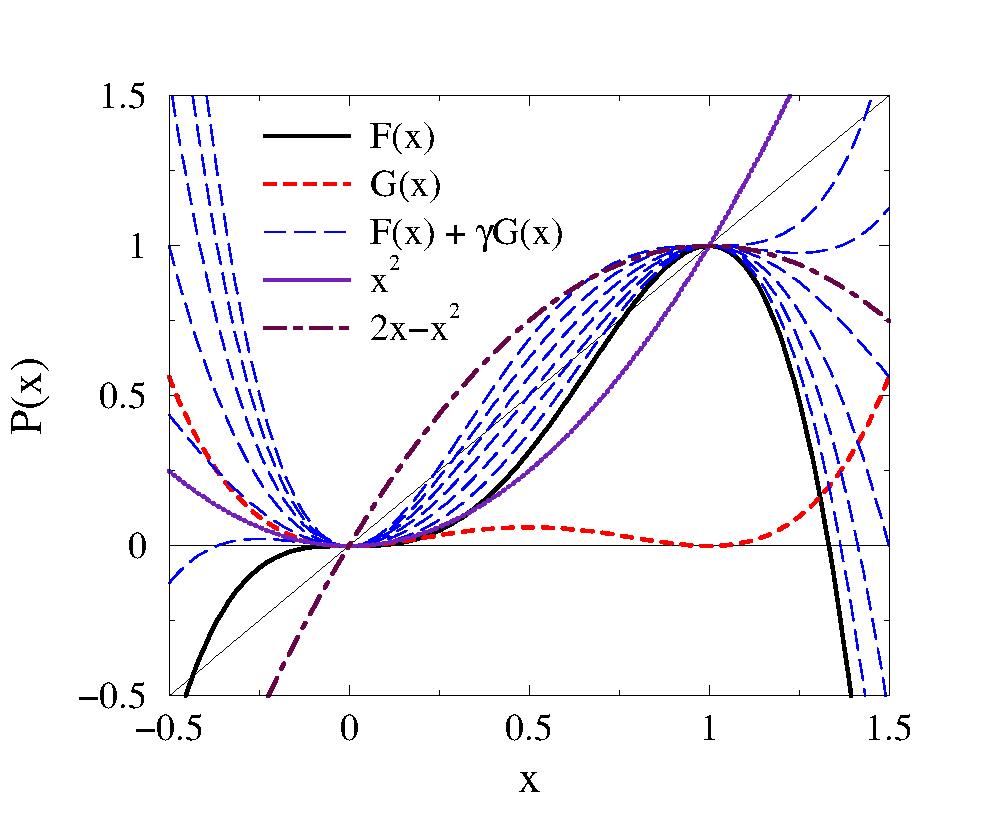
\includegraphics{TP_Fig_F_G_large.eps}
\resizebox*{3.5in}{!}{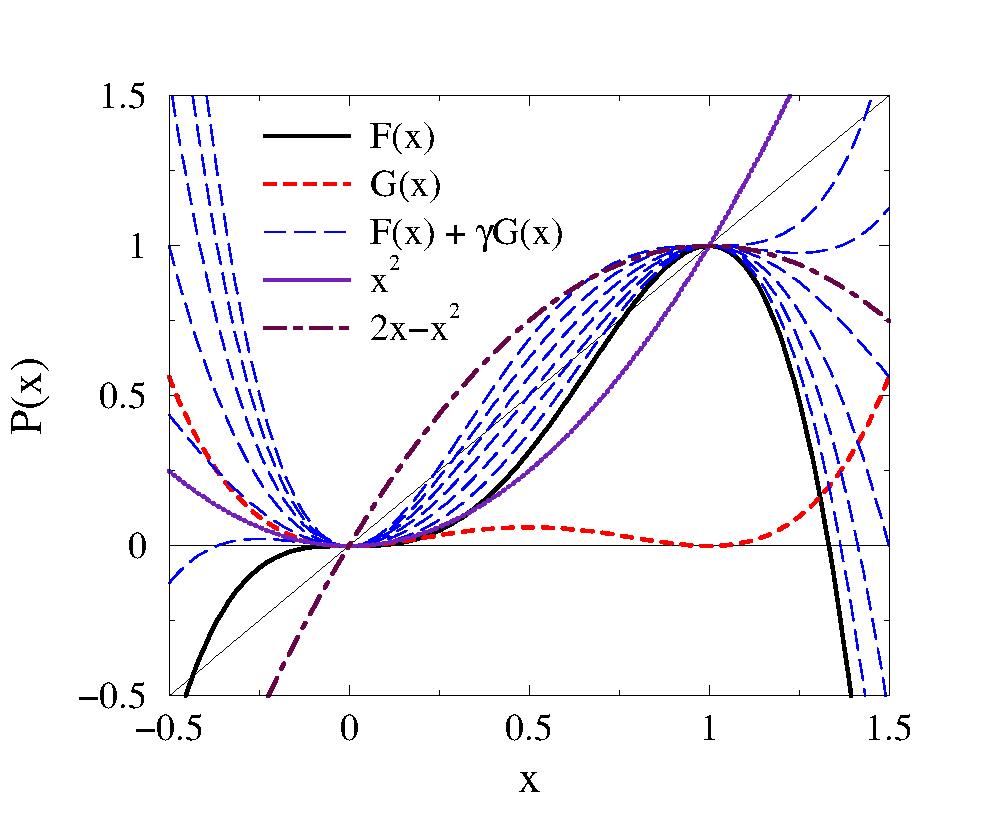
\includegraphics{TP_Fig_F_G_large.eps}}
\end{figure}
}

Trace Re-Setting (TRS) purification begins with an initial guess ${\bf X}_0$ 
with the reversed eigenvalues of ${\bf F}$ normalized to the interval $[0,1]$.
Estimates of the spectral bounds,  i.e. $\varepsilon_0({\bf F})$ and $\varepsilon_N({\bf F})$, can be computed 
by the Gersgorin bound \cite{APalser99} or more precisely with the Lanczos method \cite{ADaniels99}.  
%While the Laczos method may not be computationally expensive when carefully implemented, doing so 
%requires additional programming effort.
It is possible that due to numerical errors the Laczos estimates may not be exact bounds on
the eigenvalues, leading to instabilities in application of the SP2 functions Eq.~(\ref{sp2}) a problem
avoided with the Gersgorin upper and lower bound limits.
%In addition, the Gersgorin bound is the choice most commonly used in the literature \cite{APalser99,ADaniels99,DBowler99}.  
The slightly less efficient, but safe Gersgorin estimate has been used in the present work 
as in several in previous studies \cite{APalser99,ADaniels99,DBowler99}.
The reader should be aware however, that this approach can lead to reduced efficiencies relative 
to using the exact eigenvalues, causing a compressed shifted spectra and corresponding off-center initial 
guess for the chemical potential.  While the Trace Re-Setting method
is relatively insensitive to this error, shifting the step to the correct chemical potential can lead to substantially 
more work for the PM method in the case of high and low filling.

A general Trace Re-Setting algorithm is
\begin{equation} \label{Alg}
\begin{array}{l}
{\it function~ } {\bf P}( {\bf F}, N_e, {\it ErrorLimit})\\
{\it estimate~} \varepsilon_0({\bf F}),~\varepsilon_N({\bf F}) \\
{\bf X}_0 = (\varepsilon_{\rm N}{\bf I}-{\bf F})/(\varepsilon_{\rm N}-\varepsilon_{\rm 0}) \\
{\it while~ Error > ErrorLimit} \\
~~~ \gamma_n =(N_e - {\rm Tr} [{\cal F}({\bf X}_n ) ])/{\rm Tr} [{\cal G}({\bf X}_n ) ]\\
~~~ {\it if}~ \gamma_n  > \gamma_{\rm max}  \\
~~~ ~~~ {\bf X}_{n+1} = 2{\bf X}_n-{\bf X}_n^2\\
~~~ {\it else~ if}~ \gamma_n  < \gamma_{\rm min}  \\
~~~ ~~~ {\bf X}_{n+1} = {\bf X}_n^2 \\
~~~ {\it else}\\
~~~ ~~~ {\bf X}_{n+1} = {\cal F}({\bf X}_n) + \gamma_n  {\cal G}({\bf X}_n) \\
~~~ {\it end}\\
~~~ {\it estimate~ Error} \\
{\it endwhile}\\
{\bf P} = {\bf X}_{n+1} .
\end{array}
\end{equation}
Using the polynomials in Eq.~(\ref{FG}) leads to a quartic Trace Re-Setting (TRS4) algorithm, 
with which the remainder of this paper will be largely occupied.

To summarize, efficient spectral projections may be obtained by relaxing the 
constraint of trace conservation.  This means the extremal derivatives  may be 
different from unity, allowing a wider choice of polynomials.  The price
of this increased flexibility is mandatory resetting should the primary polynomial 
stray from its domain of convergence.  Here, we have chosen 
as the primary polynomial the quartic defined by Eq.~(\ref{FG}), with the reset
mappings supplied by the SP2 functions, Eq.~(\ref{sp2}).  However, the
Trace Re-Setting scheme presented here is a quite general framework.  We note, 
for example, that higher order generalizations can be given with 
${\cal F}_m({\bf X}) = {\bf X}^m[{\bf I} + m({\bf I} - {\bf X})]$
(for $m>2$) with ${\cal G}_m({\bf X}) = {\bf I} -{\cal F}_m({\bf I}-{\bf X})-{\cal F}_m({\bf X})$
and $\gamma \in [0,1]$. 
%
If the re-distribution step of the spectral projection SP2 is removed and if
${\cal G}({\bf X}_n)=0$, we recover grand canonical purification.
In this case the starting guess ${\bf X}_0$ must be modified with the nomalized
chemical potential $\mu({\bf X}_0) \in [0,1]$ at the inflection point of ${\cal F}(x)$.
Moreover, if the trace setting step 
${\bf X}_{n+1} = {\cal F}({\bf X}_n) + \gamma_n  {\cal G}({\bf X}_n)$ is removed
by setting $\gamma_{\rm max}=\gamma_{\rm min}=0$ and with
${\cal F}({\bf X}_n) = {\bf X}_n$ and ${\rm Tr} [{\cal G}({\bf X}_n )]=1$,
we recover the lowest order trace correcting scheme by Niklasson \cite{ANiklasson02A}.
One could also consider a more involved hierarchy of projectors, each with properties optimal 
in various regions. 
%
While not unique, it is more efficient to work with quartic polynomials than the cubics
encountered in the Mc Weeny or PM scheme, as one extra inflection may be obtained at the 
fixed points for the same number of matrix-matrix multiplications.  Optimality seems to be 
associated with polynomials of order 2, 4 and 9 \cite{ANiklasson02A}, and with achieving the 
steepest possible slope at inflection points, which is favored by 
an asymmetric polynomial \cite{ANiklasson02B}.  In the case of TRS4, the combination of 
${\cal F}$ and ${\cal G}$ is initially asymmetric, becoming symmetric at convergence as 
the McWeeny regime is reached.

\section{Thresholding, Error and Stability} \label{Error}

To achieve ${\cal O}(N)$ scaling when solving for the density matrix, sparsity 
must be enforced to prevent fill in following matrix-matrix multiplications.
The most common approach to achieving this sparsity involves an atom-atom or radial cutoff
\cite{XLi93,SQiu94,SItoh95,EHernandez95B,ACanning96}, 
beyond which matrix elements elements are not computed:
\begin{subequations}\label{CutOff}
\begin{eqnarray}
X_{\bf AB}&=&X_{\bf AB} ~~\mbox{\rm iff} ~~|{\bf A -B}| < R_{cut}\\
&=&0 ~~\mbox{\rm else},
\end{eqnarray}
\end{subequations}
allowing all matrices to employ the same graph. This technique has not been used
in the present study. Instead we use a sparse atom-blocked linear algebra \cite{MChallacombe99,MChallacombe00B},
with thresholding at the level of atom-atom blocks:
\begin{subequations}
\begin{eqnarray}
{\bf X}_{AB}&=&{\bf X}_{AB} ~~\mbox{\rm iff} ~~ ||{\bf X}_{AB} ||_F > \tau \\
&=&0 ~~\mbox{\rm else},
\end{eqnarray}
\end{subequations}
where $||\cdot||_F$ is the Frobenious norm and $\tau \in [10^{-3},10^{-6}]$ is the threshold or 
``drop tolerance''.   

A filter operation of atom-atom block thresholding is applied after every sparse matrix-matrix 
multiply to avoid fill in,
\begin{eqnarray}
{ \widetilde{ \bf X}}&=&\mbox{\tt Filter} [\bf X,\tau ] \label{filter} \\
	      &=&{\bf X}+\bm{\epsilon},\nonumber 
\end{eqnarray}
leading to the approximate matrix $\widetilde{ \bf X}$ which is in error by $\bm \epsilon$.
This can be viewed simply as a change in machine epsilon, i.e. the numerical resolution.  
In the following, we assume this error is a constant with $||\bm{\epsilon}|| \sim \tau$.

Relative to the cut-off approach, a major advantage of threshold metered sparse linear algebra 
is that it avoids discontinuities in the potential energy surface associated with atoms moving in and out 
of the cut-off radius.  Thresholding also allows for an accurate representation of the density matrix 
for systems with multiple quantum length scales, such as a nano-tube in solution or a porphyrin in a protein.
With atom-blocking, $N$-scaling is approached almost as rapidly as with element by element 
methods \cite{JMillam97,ADaniels97,ADaniels99}, while  atom-atom operations admit the use of 
dense matrix kernels such as the {\tt DGEMM} \cite{Lapack}, minimizing inefficiencies associated 
with indirect addressing and symbolic matrix overheads.  

After one matrix-matrix multiply with thresholding we have
\begin{equation}
{\widetilde{ \bf X}}^2 = {\bf X}^2 + \bm{\epsilon}\cdot {\bf X} +{\bf X} 
\cdot \bm{\epsilon}+{\cal O}(\bm{\epsilon}^2).
\end{equation}
Following this thresholding policy, repeated purification leads to an initial 
${\cal O}(  \kappa^n ||\bm{\epsilon}||)$ growth in error, where  $\kappa \gtrsim 2$ is 
a constant depending on the purification scheme.  At first glance this would seem 
an unbounded error! However,  as ${\bf X}_n$ enters the regime of quadratic 
convergence it approaches the nearly idempotent matrix ${\bf P}$.  At this point, 
the accumulation  of thresholding errors transitions from exponential to linear growth. 
For example,  $m$-fold iteration of the filtered McWeeny sequence 
close to idempotence leads to the following fixed point with weak linear drift:
\begin{equation}
{\bf P}={\bf P}+\bm{\epsilon} \cdot {\bf Q}+ (m-1){\bf P}\cdot \bm{\epsilon} \cdot{\bf Q} 
+ {\cal O}(\bm{\epsilon}^2),
\label{LinearDrift}
\end{equation}
where ${\bf Q}={\bf I}-{\bf P}$ is the virtual projector.  Thus, it is the early accumulation of 
errors preceding idempotence that are of special concern, although the  total number of 
iterations to reach convergence, $M$, is a reasonable indicator.   Recently, 
Niklasson \cite{ANiklasson02A} showed that this number scales as
\begin{equation}
\label{Mlog}
M = \alpha + \beta \log_2 \Delta g^{-1},
\end{equation}
where $\Delta g$ is the band gap at the chemical potential, and
the constants $\alpha$ and $\beta$ depend on the projection polynomial, occupancy, and
convergence goals. Assuming exponential growth, $\kappa^M$, it follows that the worst case 
accumulation errors in {\bf P} are ${\cal O}(\tau \Delta g^{-1})$.

While we can expect the deviation from idempotence, ${\bf P} - {\bf P}^2$, to be small at 
convergence, accumulation errors corrupt the commutator $[ {\bf F},{\bf P} ]$.  In addition
to raising the total energy, these commutator errors have consequences for the 
DIIS \cite{PPulay80,PPulay82} algorithm, which tries to extrapolate {\em inter-SCF} commutator 
errors to zero.  Here, incomplete sparse linear algebra leads to {\em intra-SCF} commutator 
errors that if too large can seriously corrupt the DIIS extrapolation.

\commentoutA{
\begin{figure}[t]
\resizebox*{3.5in}{!}{\includegraphics{FULL_FIGS/ConvergedC60Errors.eps}}
\caption{Behavior of the converged PM and TRS4 total energies with matrix threshold $\tau$
         for RPBE/STO-6G C60.  The log-log inset shows 
         convergence of the signed absolute error $\Delta E$ for small 
         thresholds and the line $10^{4.4} \tau^2$.}\label{c60convergence}
\end{figure}

\begin{figure}[t]
\resizebox*{3.5in}{!}{\includegraphics{XE_FIGS/xe.eps}}
\caption{The substituted zeolite Si$_{95}$TiO$_{192}$. Shown is the 0.025 isodensity surface color
mapped with the electrostatic potential. The unit cell contains the ball and stick atoms with oxygen in red,
         silicon in green and titanium not visible in this view.}\label{xefig}
\end{figure}


\begin{figure}[t]
\resizebox*{3.5in}{!}{\includegraphics{XE_FIGS/XeErrors.eps}}
\caption{Convergence of the PM and TRS4 total energies with matrix threshold $\tau$ 
         for a PBE0/STO-3G Ti substituted zeolite.  The log-log inset shows
         convergence of the signed absolute error $\Delta E$ for small 
         thresholds and the line $10^{7} \tau^2$.  Although the errors decrease monotonically, 
         quadratic convergence is not achieved until $\sim \tau = 10^{-4}$.}\label{xeerrors}
\end{figure}


\begin{figure}[tb]
\resizebox*{3.5in}{!}{\includegraphics{WATER_FIGS/WaterTimings.eps}}
\caption{CPU time for one SCF cycle of the ES, and 
	 $\tau=10^{-4}$ TRS4 and PM with number of water molecules.}\label{cputimes}
\end{figure}

\begin{figure}[tb]
\resizebox*{3.5in}{!}{\includegraphics{WATER_FIGS/ConvergedWaterErrors.eps}}
\caption{Energy per water molecule with increasing cluster size for TRS4 and PM 
         using $\tau=10^{-4}$, and by ES.}\label{waterenergyerrors}
\end{figure}

\begin{figure}[tb]
\resizebox*{3.5in}{!}{\includegraphics{WATER_FIGS/TRS4vsPMWaterCommutatorErrors.eps}}
\caption{The PM and TRS4 commutator errors $||[{\bf F ,P }]||_F$ with iteration
         at $\tau=10^{-3}, \tau=10^{-4}, \tau=10^{-5}$ and $\tau=10^{-6}$ for  
         RHF/6-31G** (H$_2$O)$_{150}$. Also shown (straight lines) are errors 
         corresponding to truncated eigensolution over the same 
         range of thresholds.}\label{commerrors}
\end{figure}

}
\section{Methods}

The PM and TRS4 algorithms were implemented in the {\sc MondoSCF}v1.0$\alpha$4, a suite of 
linear scaling Quantum Chemistry codes \cite{MondoSCF}.   All sparse matrix computations 
employed the same blocked compressed sparse row (BCSR) \cite{MChallacombe99,MChallacombe00B,MChallacombe03B} 
data structure.  With the BCSR data structure, the cost of recomputing the symbolic matrix 
is negligible, allowing dynamic fill-in.  The BCSR-BCSR multiplies are carried with 
small dense matrix-matrix multiplies ({\tt DGEMM}s) that have been written in highly optimized 
platform specific C by {\sc PHiPAC} \cite{Bilmes96a,Bilmes97b,PHiPAC} for blocks in the range 
3x3x3 to 15x15x15. 

The code was compiled using the Portland Group F90 compiler {\sc pgf90}v3.2.4 \cite{pgf90} with 
the {\tt -O1 -tp athlon} options  and with the gnu C compiler {\sc gcc}v2.96 using the {\tt -O1} flag.  
All calculations were carried out on a 1.2GHz AMD Athlon Thunderbird running RedHat 
{\sc Linux}v7.3 \cite{RedHat73}.  Exact eigensolution (ES) was carried out with the native
{\sc DSYEV} and {\sc BLAS} {\sc LAPACK} routines supplied with {\sc pgf90}.

Filter operations were carried out after every matrix-matrix multiply, unless the product
participates in a sum, in which case thresholding was postponed.  The TRS4 algorithm of 
Eq.~(\ref{Alg}) was implemented as follows
\begin{subequations} 
\begin{eqnarray}
&&{\bf X}_{n+1} = {\tt Filter}[{\bf X}^2_n,\tau], ~~~~~~~~~~~~~~ \mbox{or} \\
&&{\bf X}_{n+1} = {\tt Filter}[2{\bf X}_n -{\bf X}^2_n,\tau], ~~~~~ \mbox{or} \\[0.2cm]
&&{\bf Y}=\gamma_n {\bf I}+ (4-2\gamma_n){\bf X}_n + (\gamma_n-3){\bf X}^2_n \nonumber\\
&&{\bf X}_{n+1} = {\tt Filter}[\widetilde{\bf X}^2_n \widetilde{\bf Y},\tau]. \label{trs4filter} 
\end{eqnarray}
\end{subequations}
In Eq.~(\ref{trs4filter}), truncation occurs post-summation with a tilde indicating filtered objects.

All ES calculations employed L{\"o}wdin symmetric orthogonalization \cite{PLowdin50,PLowdin56}, 
while all TRS4 and PM calculations used the congruence transformation provided by incomplete 
inverse Cholesky factors calculated with sparse atom-blocked AINV \cite{MChallacombe99,MBenzi01,MChallacombe03B}.
The exception is chlorophyll, which due to severe ill-conditioning in the largest basis sets, demanded symmetric 
orthogonalization.

Unless otherwise stated, all errors in eigensolution of the SCF equations correspond to 
truncation of the density matrix with $\tau=10^{-6}$.  This is taken as a reference, and will be
referred to in the following as eigensolution (ES).  No variable thresholding, fitting functions,
fixed-form sparse matrices or incremental Fock builds were used in any experiments.  Thresholds 
controlling other linear scaling approximations, such as 
AINV \cite{MChallacombe99,MBenzi01,MChallacombe03B}, 
HiCu \cite{MChallacombe00A,CGan03},  
QCTC \cite{MChallacombe96,MChallacombe96B,MChallacombe97,MChallacombe03A}, or
ONX \cite{ESchwegler96,ESchwegler97,ESchwegler98A,ESchwegler98C,ESchwegler99,ESchwegler00}
were set to ``tight''  which, in the absence of accumulation errors, allow SCF convergence to within 
$\delta E < 10^{-9}$ (relative error in the total energy ) and 
$\Delta{\bf P} < 10^{-5}$ (maximum absolute error in a density matrix element). In the following, all 
experiments seek to meet these accuracy goals.  However, tweaking $\tau$  can lead to intra-SCF commutator 
errors (discussed in Section~\ref{Error}), possibly corrupting DIIS extrapolation \cite{PPulay80,PPulay82} and 
causing it to stall before meeting the accuracy goals.  Stagnation of the DIIS is detected by 
the code, leading to termination of the SCF.

\section{Results}

A comparison is made between quartic Trace Re-Setting (TRS4), Palser-Manolopoulos \cite{APalser99}  
(PM) and exact truncated eigensolution (ES) in both the high and low filling regimes, where we expect 
TRS4 to have a significant advantage over PM.

\smallskip
Atomic units are used throughout. 

\subsection{High Filling}

Of special concern is the behavior of linear scaling methods in the high filling limit,
as this is the regime that allows the most convenient access to large systems through
tight-binding, semi-empirical and minimal basis {\em ab initio} methods.
This concern is underscored by Ref.~\onlinecite{ADaniels99}, in which Daniels and Scuseria 
found the PM method to be unstable for semi-empirical calculations on C60 requiring  
$\approx 100$ SCF cycles and level shifting to avoid excited state solutions.
Also, Bowler has found that by itself, the PM method with the radial cut-off approximation 
is encumbered by an error too large for non-self-consistent tight-binding calculations \cite{DBowler99}.  
In the following,  convergence of PM and TRS4 with $\tau$ is explored for self-consistent model 
chemistries applied to minimal basis C60 and a Ti substituted zeolite.

\subsubsection{C60}

Calculations on C60 were carried out at the RPBE/STO-6G level of theory, converging the
SCF using PM and TRS4 with matrix thresholds $\tau \in [10^{-2},10^{-5}]$.  
Convergence of the total energy with matrix threshold is shown in Fig.~\ref{c60convergence}.  The inset contains 
the signed absolute errors $\Delta E$ relative to the ES total energy $E_{\rm ES}=-2278.116$ 
and the fit $10^{4.4} \tau^2$.  While more SCF cycles were required for loose thresholds ($\tau > 10^{-4}$), 
all calculations converged in less than 16 cycles and the PM and TRS4 energies approach 
quadratically from above as $\tau$ is tightened.  Consistent with the filling $f_{\rm occ}=0.62$, no dramatic
differences are found between the two methods; $M_{\rm PM}/M_{\rm TRS4} \approx 1.2$ and 
$M_{\rm TRS4}=38$ for $\tau=10^{-5}$.   

\subsubsection{Titanium Substituted Zeolite}

A higher filling, $f_{\rm occ}=0.8$, is encountered with a minimal basis and the titanium substituted zeolite 
Si$_{95}$TiO$_{192}$.  Periodic boundary conditions were implemented as described in Ref.~\onlinecite{CTymczak03}.    
The zeolite geometry was relaxed using TRS4 with $\tau = 10^{-5}$ at the PBE/STO-3G level
\commentoutB{.}
\commentoutA{, and is shown in Fig.\ref{xefig}.} 
Calculations on this zeolite were then carried out at the PBE0/STO-3G level of theory,  
converging the SCF using PM and TRS4 with matrix thresholds $\tau \in [10^{-2},10^{-5}]$.  
Convergence of the total energy with matrix threshold is shown in Fig.~\ref{xeerrors}.  The inset contains 
the signed absolute errors $\Delta E$ relative to the ES total energy $E_{\rm ES}=-42253.199$ and the line 
$10^{7} \tau^2$.  While always decreasing with $\tau$, the error doesn't reach a smooth quadratic convergence 
until $\approx \tau < 10^{-4}$.  With a larger filling factor, the differences between PM and TRS4 are more 
significant than in the case of C60, with $M_{\rm PM}/M_{\rm TRS4} \approx 2.2$ and $M_{\rm TRS4}=35$ for $\tau=10^{-5}$.  
Also, differences in errors between the two methods are more pronounced as shown in Fig.~\ref{xeerrors}

\subsection{Low Filling}

The low filling limit is less commonly employed in linear scaling studies.  However, as parallel versions
of ${\cal O}(N)$ Quantum Chemistry programs become available \cite{MChallacombe00B,CGan03}, this regime 
is certain to become accessed with more regularity.  We consider two systems.  The already well benchmarked 
system of water clusters at the RHF/6-31G** level of theory, and basis set progression for Chlorophyll.

\subsubsection{Water}

Differences between PM, TRS4 and ES were explored using a sequence of water clusters
\cite{MChallacombe96,MChallacombe96A,MChallacombe97,JBurant96,ESchwegler97,JMillam97,ADaniels97,COchsenfeld98,ESchwegler99}, 
(H$_2$O)$_{10}$ through (H$_2$O)$_{150}$, at the RHF/6-31G** level of theory. The ability to reach the regime 
of true linear linear scaling with this basis set is demonstrated in Fig.~\ref{cputimes}.
Crossover with ES occurs at about 50 water molecules, with {\sc TRS4} and {\sc PM} achieving a sustained 
performance better than 400 Mflop/s.  Despite low filling, $f_{\rm occ}=0.2$, and the fact that PM 
requires 30 iterations to converge while TRS4 takes only 18, the ratio of cpu times is only 1.2.  
This is because the PM method involves intermediate matrices that fill-in more slowly, leading to 
faster sparse matrix-matrix multiplies and a fairly dramatic difference in errors.  
This difference is shown in Fig.~\ref{waterenergyerrors}, where PM, TRS4 and ES energies per water molecule 
are compared over increasing cluster size.  As argued in Section~\ref{Error}, accumulation errors 
in the density matrix scale as $||{\bm\epsilon}||\sim \tau$. This is clearly demonstrated in 
Fig.~\ref{commerrors}, which shows decade by decade control over the commutator error 
$||[{\bf F,P}]||_F$ for PM, TRS4 and truncated eigensolution (pure truncation error) with $\tau$. 
In each case, the TRS4 errors are approximately one order of magnitude larger than those due to 
truncation, while the PM errors are about two orders larger.  Also, note an initial exponential  
increase in the errors, as discussed in Section~\ref{Error}, followed by stabilization at
idempotency convergence (and a small linear rise detectable only with the most liberal threshold).

\subsubsection{Chlorophyll}
 
To study the low filling regime more carefully, basis set progression of ES, PM 
and TRS4 was carried out for chlorophyll, a relatively small (91 atom) Mg containing porhyrin ring system. 
A tight,  $\tau=10^{-6}$ matrix threshold was used throughout.  Symmetric L\"owdin orthogonalization 
was used due to high condition numbers $\sim 10^9$ arising from the extended basis sets, which 
our current version of AINV was unable to cope with.  In Table~\ref{ChlorophyllConvergence}, 
total energies computed with ES, the number of matrix-matrix multiplies and the absolute signed 
error in the total energies of PM and TRS4 are presented.  Although the initial guess ${\bf X}_0$ 
in these studies is typically $\approx 99\%$ dense, PM takes a more sparse path towards convergence, 
dropping to $\approx 90\%$ full.  Also, as the basis set size increases so does the number 
of matrix-matrix multiplies $M_{\rm PM}$ required for PM to reach convergence. For the 
larger basis sets the behavior of PM becomes pathological,  leading to errors greater 
than a $m$hartree even with quite a tight threshold.  On the other hand, the TRS4 accumulated error 
remains stable at about 0.1 $\mu$hartree.
\commentoutA{
\begin{table}[h]
\caption{Basis set progression of ES, PM and TRS4 values for RPBE chlorophyll with $\tau = 10^{-6}$, including 
matrix-matrix multiplies $M$ to convergence, order of the signed absolute error in the converged total 
energy $\Delta E$, and the ES total energy.}
\label{ChlorophyllConvergence}
\squeezetable
\begin{tabular}{lcccccc}
\toprule
Basis set       &  $f_{\rm occ}$ & $E_{\rm ES}$       &$M_{\rm PM}$&$M_{\rm TRS4}$& $\Delta E_{\rm PM}$ & $\Delta E_{\rm TRS4}$ \\
\colrule
STO-3G          &  0.62      & -2348.268  & 63      & 45       & $ 10^{-6}$   &  $ 10^{-7}$   \\ 
3-21G           &  0.34	     & -2365.182  & 59      & 47       & $ 10^{-6}$   &  $ 10^{-8}$   \\
Ahlrichs VDZ    &  0.34      & -2375.971  & 59      & 43       & $ 10^{-7}$   &  $ 10^{-8}$   \\
6-31G**         &  0.19      & -2378.313  & 75      & 48       & $ 10^{-6}$   &  $ 10^{-7}$   \\
Ahlrichs VTZ    &  0.21      & -2378.400  & 107     & 57       & $ 10^{-3}$   &  $ 10^{-7}$   \\
6-311G**        &  0.15      & -2378.853  & 115     & 55       & $ 10^{-4}$   &  $ 10^{-7}$   \\
6-311G(2d,2p)   &  0.11      & -2378.930  & 147     & 61       & $ 10^{-3}$   &  $ 10^{-8}$   \\
\botrule
\end{tabular}
\end{table}
}
\section{Discussion}

In a recent World Technology Evaluation Center report on molecular modeling \cite{WTECMM02}, 
Stechel noted that when it comes to the success of linear scaling  methods 
``the devils are in the details''.  This paper has tried to articulate these details for
purification methods, making clear the interplay between iterative density matrix solver and
incomplete sparse linear algebra, consequences of high and low filling basis sets and the 
impact of commutator errors on SCF acceleration. 

Minimizing the number of matrix-matrix multiplies to achieve idempotence is a key factor in reducing
accumulation errors, with TRS4 a clear improvement over PM for basis sets in both the high and 
low filling regime where PM behaves poorly.  This poor behavior stems from domination by 
either the virtual or occupied space, skewing the PM polynomial to form a step close to 0
or 1 where it looses efficiency.  In some cases, this effect is undoubtedly magnified by the 
inaccurate Gersgorin estimate, which may shift and compress the Fockian eigenspectrum.  We 
have chosen not to explore this latter effect as the basic deficiency in PM remains, and 
TRS4 does not suffer from either problem, while also overcoming potential problems with 
degeneracy and fractional occupancy as discussed in Appendix~\ref{Degen}.

As shown in Fig.~\ref{waterenergyerrors}, using TRS4 and $\tau=10^{-4}$ for a large gap system 
leads to  early crossovers with eigensolution and true linear scaling at an energetic 
cost of about 0.1 mhartree per heavy atom.  This cost is akin to a change of basis, 
as matrix truncation limits the variational space, 
corrupting the commutator $[{\bf F,P}]$ and raising the total energy.  While accumulation 
errors due to purification are distinct from truncation errors, their combined effect is the 
same, leading to corruption of the commutator and raising the energy.   

Although system dependent, variation of thresholds with $\tau \lesssim 10^{-4}$ typically leads to a 
linear decrease in the commutator error, as in Fig.~\ref{commerrors}, and corresponding
${\cal O}(\tau^2)$ errors in the total energy that approach the ES value from above as shown
in Figs.~\ref{c60convergence} and \ref{xeerrors}.  For more higher values of $\tau$, the 
shrinking pool of large atom-atom blocks leads to discretization of the error curve.  
Nevertheless, errors in this regime decrease monotonically with $\tau$, and as self-consistency 
is reached the iterations to idempotence and the graph of the density matrix stabilize at 
convergence, yielding a well defined variational approximation.

One concern with purification methods is that toward idempotence, the electronic energy 
fails to decrease monotonically \cite{DBowler99,APalser99} due to incomplete linear algebra.  
This corresponds to fixed point convergence of the density matrix, as given 
by Eq.~(\ref{LinearDrift}), followed by a weak linear increase in error.  However, this small 
linear error growth is of little concern as the initial exponential accumulation of errors 
completely dominates.  
%{\bf
%The picture is different for non-variational methods under severe truncation,
%where error growth in the density matrix following idempotence may involve higher order error terms, 
%${\cal O}(\bm \epsilon^2)$,  leading to unacceptable first order errors in the total energy 
%$\delta E \sim {\rm Tr} {\bf F} \delta \bf P$.}

For more liberal thresholds, errors in the commutator can lead to poor performance
of the DIIS.  While DIIS has been used throughout this work with stall induced termination of 
the SCF, simple damping often yields a more stable and rapid convergence in this regime.  Thus, 
there is a need for extrapolation algorithms that can accommodate commutator errors.  For more 
conservative thresholds, the conventional DIIS algorithm becomes more reliable, resulting in convergence 
comparable to that obtained with conventional (dense) methods.  In production, $\tau=10^{-4}$ is considered 
``loose'' and $\tau=10^{-6}$ ``tight'' for large to medium gap systems.  

Quartic Trace Re-Setting is a clear improvement over the PM method in both the high 
($f_{\rm occ}\gtrsim 0.8$) and low ($f_{\rm occ} \lesssim 0.2$) filling regimes,  typically requiring
less than half the matrix-matrix multiplies required by PM.  With thresholding, the expected performance 
increase is not realized, as PM tends to employ intermediate matrices that are sparser.  
However, the larger number of sparse matrix-matrix multiplies employed by PM leads to a dramatically larger 
accumulation of errors, shown in Figs.~\ref{xeerrors} and \ref{waterenergyerrors}, exceeding an order of 
magnitude for basis sets that can readily access the linear scaling regime.
For bigger basis sets,  TRS4 is up to four orders of magnitude more accurate than PM as listed in 
Table.~\ref{ChlorophyllConvergence}.  Although low filling is intrinsic to semi-empirical and tight-binding methods, 
minimal basis sets are of limited value in {\em ab initio} studies.  However, recent studies have shown that with 
{\em in situ} basis set optimization \cite{EHernandez95,MLee97,JTalman01,GBerghold02}, significantly improved results may 
be achieved with a reduced representation.  Also, parallel implementations of ${\cal O}(N)$ 
methods \cite{MChallacombe99,CGan03} will soon allow access to the large basis set regime for large scale 
calculations.


\begin{acknowledgments}
This work has been carried out under the auspices of the US Department 
of Energy under contract W-7405-ENG-36 under the ASCI project.
\end{acknowledgments}

\bibliographystyle{apsrmp}
\bibliography{mondo}

\appendix

\section{Degeneracy}\label{Degen}

One advantage with the Trace Re-Setting scheme and the trace
conserving PM scheme, compared to some variational schemes \cite{XLi93}
and the grand canonical purification method,
are their ability to deal with degeneracy and fractional occupancy.
Below we briefly discuss the problem with degeneracy and fractional
occupancy, how they destroy idempotence and how they can be calculated
from the density matrix.

Consider the density matrix ${\bf P}$  with a $\nu$ fold degeneracy
and $n_d$ occupied degenerate states. The trace of the density matrix can be written
\begin{equation}
Tr [ {\bf P}  ] = N_e = N_e-n_d + \nu \tau,
\end{equation}
where $\tau = n_d/\nu$ is the filling of the degenerate states.
In the case of fractional filling of a non-degenerate state at the
chemical potential $\nu = 1$ and $\tau = n_d < 1$,
the density matrix is, by analogy with Eq. (\ref{Density}),
\begin{equation}\label{Density}
{\bf P} = \sum_{k=1}^{N_{\rm el}-n_d} {\bf c}^{\rm T}_{k} {\bf c}_{k} +
 \sum_{k=N_{\rm el}-n_d +1}^{N_{\rm el}- n_d + \nu } \tau {\bf c}^{\rm T}_{k} {\bf c}_{k}
\end{equation}
and with an orthogonal representation we have that
\begin{equation}
{\bf P}^m = \sum_{k=1}^{N_{\rm el}-n_d} {\bf c}^{\rm T}_{k} {\bf c}_{k} +
 \sum_{k=N_{\rm el}-n_d +1}^{N_{\rm el}- n_d + \nu } \tau^m {\bf c}^{\rm T}_{k} {\bf c}_{k}.
\end{equation}
For powers of the density matrix we thus have that
\begin{equation} \label{Rhom}
{\rm Tr} [ {\bf P}^m  ] = N_{\rm el} - n_d + \nu \tau^m \neq Tr  [ {\bf P} ] = N_{\rm el}.
\end{equation}
From Eq.\ (\ref{Rhom}) we see that idempotence is not
fulfilled (when $m>1$) in the case of degeneracy or fractional filling. 
This means, for example, that grand canonical purification does not work and
that the McWeeny constraint in conjugate gradient
minimization schemes cannot be applied \cite{XLi93}.
In order to achieve a constrained search also
in the degenerate case the trace imposing polynomials
${\cal F}({\bf X}) + \gamma {\cal G}({\bf X})$ above, or the trace conserving polynomials
in the canonical PM scheme may possibly be used as alternatives.

Equation (\ref{Rhom}) can be used, as long as
$n \neq \nu$, to calculate the degenerate filling factor and the degeneracy.
Solving the equations (with $m=1,2,3$) for the degeneracy and occupancy
of the degenerate states we get
\begin{equation}
n_d = \frac{({\rm Tr} [{\bf P}-\rho_0^2 ])^2}{{\rm Tr} [{\bf P}-2{\bf P}^2+{\bf P}^3 ]},
\end{equation}
\begin{equation}
\nu = \frac{({\rm Tr} [{\bf P}-{\bf P}^2 ])^3}{{\rm Tr} [{\bf P}^2-{\bf P}^3 ]
{\rm Tr} [{\bf P}-2{\bf P}^2+{\bf P}^3 ]}
\end{equation}
and
\begin{equation}
\tau = \frac{{\rm Tr} [{\bf P}^2-{\bf P}^3 ]}{{\rm Tr} [{\bf P}-{\bf P}^2 ]}.
\end{equation}
These formulas can be viewed as alternative conditions to idempotence
for a degenerate density matrix or in the case of fractional occupancy. 
The relations can also be used
to derive the value of $\gamma_n$ at convergence. For the particular
choice of functions $\cal F$ and $\cal G$ above, Eq.\ (\ref{FG}), we have that
\begin{equation}
\lim_{n \rightarrow \infty} \gamma_n = \frac{n_d - \nu {\cal F}(\tau )}
                                               {\nu {\cal G}(\tau )}.
\end{equation}
Notice, that if $\gamma_{\infty}$
is outside its bounds of stability, i.e.\ if $\gamma_{\infty} \notin [0,6]$, we cannot deal with
degeneracy and fractional filling. The scheme will still
converge, but not to the correct density matrix. For example,
a 100 folded degeneracy requires $n_d \in [24,76]$ otherwise
$\gamma$ will be out of bound at convergence. This puts some
limitations on the ability to treat degeneracy and fractional filling
with the proposed Trace Re-Setting algorithm.


\commentoutB{

\clearpage

\begin{center}
\bf  TABLES\\[1.cm]
\end{center}


\begin{table}[h]
\caption{Basis set progression of ES, PM and TRS4 values for RPBE chlorophyll with $\tau = 10^{-6}$, including 
matrix-matrix multiplies $M$ to convergence, order of the signed absolute error in the converged total 
energy $\Delta E$, and the ES total energy.}
\label{ChlorophyllConvergence}
\squeezetable
\begin{tabular}{lcccccc}
\toprule
Basis set       &  $f_{\rm occ}$ & $E_{\rm ES}$       &$M_{\rm PM}$&$M_{\rm TRS4}$& $\Delta E_{\rm PM}$ & $\Delta E_{\rm TRS4}$ \\
\colrule
STO-3G          &  0.62      & -2348.268  & 63      & 45       & $ 10^{-6}$   &  $ 10^{-7}$   \\ 
3-21G           &  0.34	     & -2365.182  & 59      & 47       & $ 10^{-6}$   &  $ 10^{-8}$   \\
Ahlrichs VDZ    &  0.34      & -2375.971  & 59      & 43       & $ 10^{-7}$   &  $ 10^{-8}$   \\
6-31G**         &  0.19      & -2378.313  & 75      & 48       & $ 10^{-6}$   &  $ 10^{-7}$   \\
Ahlrichs VTZ    &  0.21      & -2378.400  & 107     & 57       & $ 10^{-3}$   &  $ 10^{-7}$   \\
6-311G**        &  0.15      & -2378.853  & 115     & 55       & $ 10^{-4}$   &  $ 10^{-7}$   \\
6-311G(2d,2p)   &  0.11      & -2378.930  & 147     & 61       & $ 10^{-3}$   &  $ 10^{-8}$   \\
\botrule
\end{tabular}
\end{table}

\clearpage

\begin{figure}[h]
\begin{center}
\bf  FIGURES\\[1.cm]
\end{center}

\caption{Examples of spectral projection polynomials $P(x) = F(x) + \gamma G(x)$
for different values of the adjustment factor $\gamma \in [0,6]$.} \label{Fig_F_G}

\caption{Behavior of the converged PM and TRS4 total energies with matrix threshold $\tau$
         for RPBE/STO-6G C60.  The log-log inset shows 
         convergence of the signed absolute error $\Delta E$ for small 
         thresholds and the line $10^{4.4} \tau^2$.}\label{c60convergence}

\caption{Convergence of the PM and TRS4 total energies with matrix threshold $\tau$ 
         for a PBE0/STO-3G Ti substituted zeolite.  The log-log inset shows
         convergence of the signed absolute error $\Delta E$ for small 
         thresholds and the line $10^{7} \tau^2$.  Although the errors decrease monotonically, 
         quadratic convergence is not achieved until $\sim \tau = 10^{-4}$.}\label{xeerrors}

\caption{CPU time for one SCF cycle of the ES, and 
	 $\tau=10^{-4}$ TRS4 and PM with number of water molecules.}\label{cputimes}

\caption{Energy per water molecule with increasing cluster size for TRS4 and PM 
         using $\tau=10^{-4}$, and by ES.}\label{waterenergyerrors}

\caption{The PM and TRS4 commutator errors $||[{\bf F ,P }]||_F$ with iteration
         at $\tau=10^{-3}, \tau=10^{-4}, \tau=10^{-5}$ and $\tau=10^{-6}$ for  
         RHF/6-31G** (H$_2$O)$_{150}$. Also shown (straight lines) are errors 
         corresponding to truncated eigensolution over the same 
         range of thresholds.}\label{commerrors}
\end{figure}

\clearpage

\begin{center}
Figure 1, A.~Niklasson,  C.~J.~Tymczak and M.~Challacombe \\[1.cm]
\resizebox*{7in}{!}{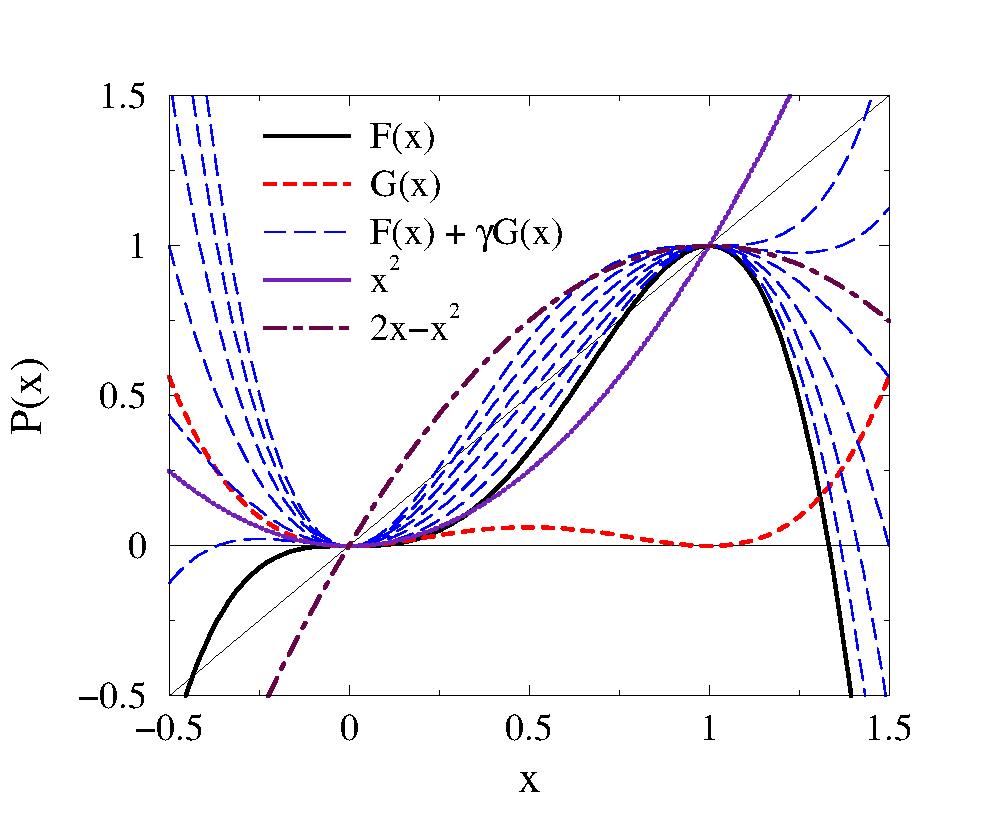
\includegraphics{TP_Fig_F_G_large.eps}}
\end{center}

\clearpage

\begin{center}
Figure 2, A.~Niklasson,  C.~J.~Tymczak and M.~Challacombe \\[1.cm]
\resizebox*{7in}{!}{\includegraphics{FULL_FIGS/ConvergedC60Errors.eps}}
\end{center}

\clearpage

\begin{center}
Figure 3, A.~Niklasson,  C.~J.~Tymczak and M.~Challacombe \\[1.cm]
\resizebox*{7in}{!}{\includegraphics{XE_FIGS/XeErrors.eps}}
\end{center}

\clearpage

\begin{center}
Figure 4, A.~Niklasson,  C.~J.~Tymczak and M.~Challacombe \\[1.cm]
\resizebox*{7in}{!}{\includegraphics{WATER_FIGS/WaterTimings.eps}}
\end{center}

\clearpage

\begin{center}
Figure 5, A.~Niklasson,  C.~J.~Tymczak and M.~Challacombe \\[1.cm]
\resizebox*{7in}{!}{\includegraphics{WATER_FIGS/ConvergedWaterErrors.eps}}
\end{center}

\clearpage

\begin{center}
Figure 6, A.~Niklasson,  C.~J.~Tymczak and M.~Challacombe \\[1.cm]
\resizebox*{7in}{!}{\includegraphics{WATER_FIGS/TRS4vsPMWaterCommutatorErrors.eps}}
\end{center}

}

\end{document}
